\documentclass[10pt]{article}
\usepackage[margin=0.7in]{geometry}
\usepackage{amsmath,amssymb,graphicx,booktabs,hyperref}
\hypersetup{colorlinks=true,linkcolor=blue,urlcolor=blue}
\title{Finite Semaev row-space closure audit}
\author{Independent finite-model validation}
\date{26 October 2026}
\begin{document}
\maketitle

\noindent\textbf{Status.} This is a scoped computational audit of one frozen
Boolean draw. It does not change a Lean theorem, formal target, experiment
output, official hypothesis status, or ECDLP cost claim. The executable
checker and exact machine-readable output are beside this PDF as
\texttt{audit.py} and \texttt{evidence.json}.

\section*{Question and sources}
Does the selected degree-three row span of the fixed
$n=4,n'=4,s=1,x_R=1$ Semaev $S_3$ system satisfy the multiplication closure
needed to identify it with a $V_{F,3}$ filtration? The archived equation hash
is recorded in \texttt{evidence.json}. The repository sources are
\texttt{research/FFD\_SEMAEV\_MEASUREMENT1.md}, the corrected replay of
22 October, and the finite Lean row-space certificates. The relevant
mathematical boundary is the degree-budget closure definition in
\href{https://arxiv.org/pdf/2112.05579}{Caminata--Gorla, Definition 1.5}.
\href{https://arxiv.org/pdf/1503.08001}{Kosters--Yeo, Corollary 4.11 and
Remark 4.12} give the trace identity and describe degree-two first falls as
usual, rather than universal under every factor-base choice.

\section*{Reproduction and controls}
The checker independently evaluates $S_3=e_2^2+e_3+1$ on all 256 Boolean
assignments over $\mathbb{F}_2[X]/(X^4+X+1)$, then uses a M\"obius transform
to recover all four archived component equations. It confirms that $x_R=1$
is the abscissa of curve points with $y=6$ and $y=7$. Boolean products use
OR on variable masks and XOR on coefficients. A strict multiplier-degree
budget and the historical actual-product-degree row selector yield the same
rank and top-degree projection rank for this sample:

\begin{center}
\begin{tabular}{rrrrr}
\toprule
Degree & Strict rows & Product-degree rows & Rank & Projection rank\\
\midrule
1 & 1 & 17 & 1 & 1\\
2 & 12 & 28 & 11 & 10\\
3 & 64 & 80 & 53 & 41\\
\bottomrule
\end{tabular}
\end{center}

\noindent The archived 80-draw chart is preserved. The additive chart below
labels its 68/12 corrected outputs as \emph{direct-row grades}; their
identification with a closed-filtration first-fall count is unverified.

\section*{Closure witness and limit}
The published degree-two witness $W$ belongs to the selected rank-53
degree-three span and lies outside the selected degree-two span. Multiplying
by $u_0$ gives a degree-three polynomial outside that rank-53 span; adjoining
it raises the rank to 54. Since $\deg W=2$ and $\deg u_0=1$, the selected
degree-three span is not closed under this Boolean-quotient degree-budget
product. This does \emph{not} invalidate the Lean theorem about the literal
80 rows. It shows that a separate bridge is needed before calling that span
the full closed $V_{F,3}$ filtration. The rank of the complete closed
filtration and the polynomial-ring/Boolean-quotient correspondence are not
established here. A reviewed definition and a Lean closure or corrected-row
certificate are the next proof obligations.

\noindent\textbf{Operational limit.} No heavy Lean build was started. GitHub
Actions reports a payment-or-spending-limit condition before assigning
runners, and the Spot host lacks the required 16 GiB reserve for a heavy
local build. The complete report with source links and exact witness masks is
in \texttt{report.md}.

\clearpage
\begin{figure}[!ht]
\centering
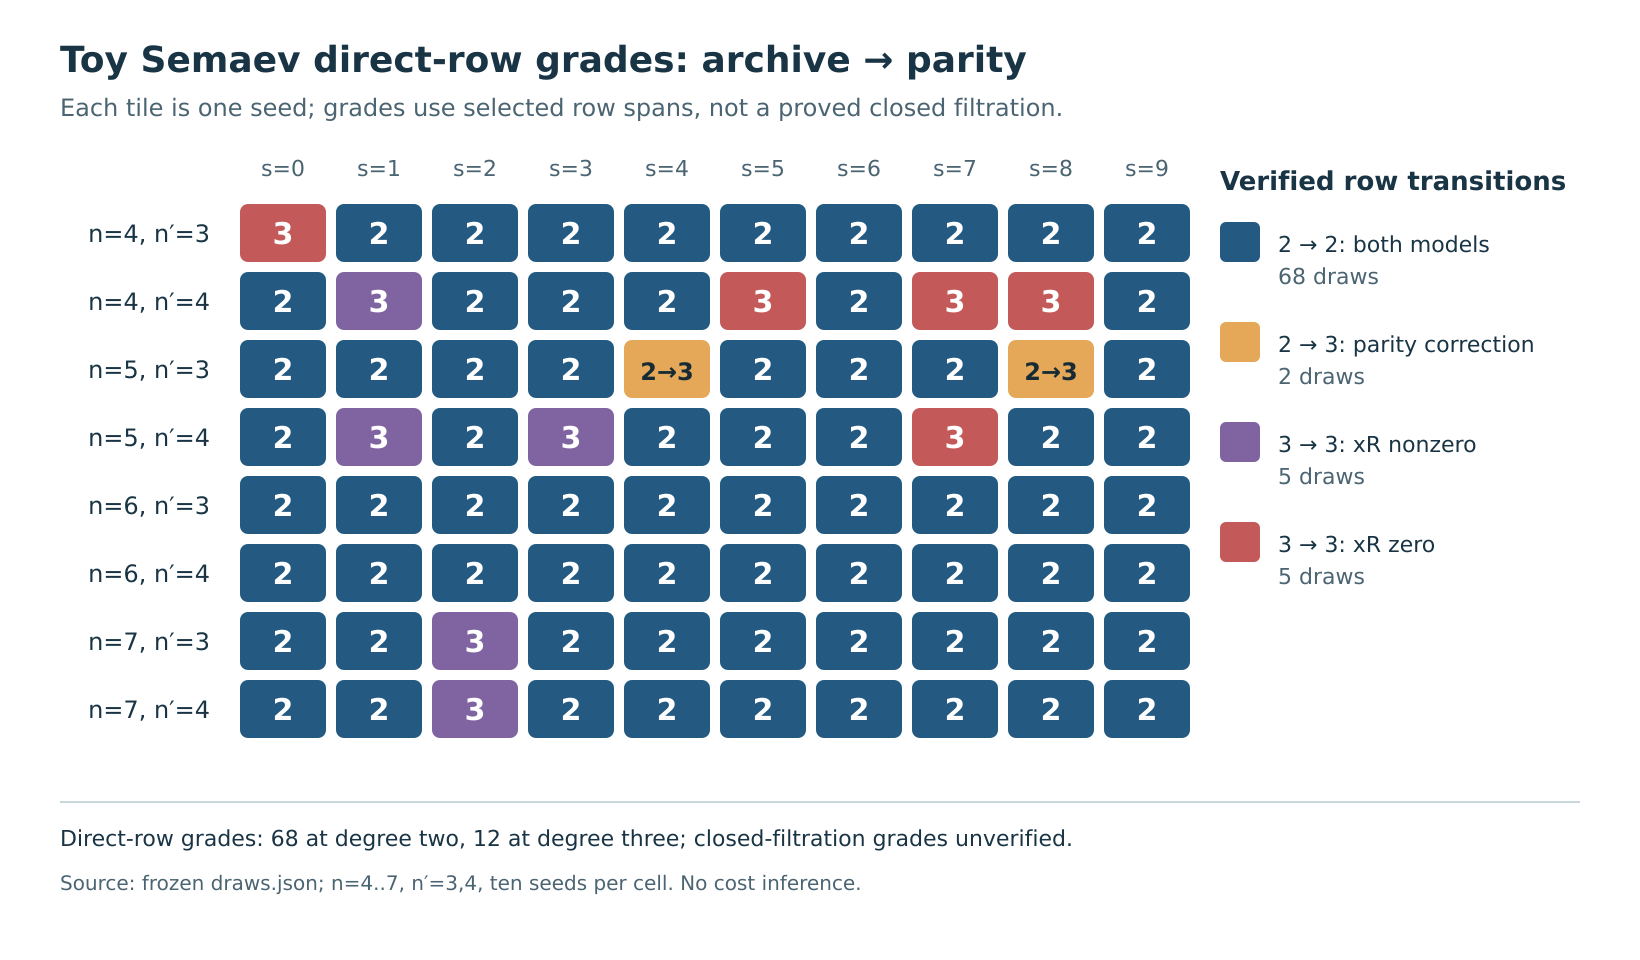
\includegraphics[width=0.94\textwidth]{direct-row-grades.png}
\caption{Archived set-product and parity-corrected direct-row grades for
eight fixed cells of ten draws. The renderer verifies all 80 tiles against
the archived SVG. This is neither a timing plot nor an attack-cost result.}
\end{figure}
\end{document}
